%%%%%%%%%%%%%%%%%%%%%%%%%%%%%%%%%%%%%%%%%%%%%%%%%%%%%%%%%%%%%%%%%%%%%
%                                                                   %
% Cette version repart de 03_Draft\figures_tables-short-current.tex %
%                                                                   %
%%%%%%%%%%%%%%%%%%%%%%%%%%%%%%%%%%%%%%%%%%%%%%%%%%%%%%%%%%%%%%%%%%%%%

% Moved from the appendix (former Table A4) in the R2 revision, in response to Referee 3's point 1.
\begin{table}[h!]\caption{Descriptive statistics before displacement: displaced workers (LE) and matched controls}\label{tab:desc:AllLE}
	\begin{center}
		% Generated from current results_analysis CSV files by master.R, section I (scripts/I-PLOTS_AND_TABLES).
% Table 1; status: ready
% Normalized differences recomputed using pooled SD; hourly-wage means and SDs use the updated exports.
% -- means a requested statistic is unavailable; an empty cell means not applicable.
{
\begin{tabular}{lccc}
\hline\hline
 & (1) & (2) & (3) \\
 & LE & Control & Norm. Diff. \\
\hline
\multicolumn{4}{l}{\textbf{Matching variables}} \\
Age & 37.05 & 37.01 & +0.005 \\
 & (8.04) & (8.09) &  \\
Hourly wage at $t^D-2$ & 14.91 & 14.92 & -0.001 \\
 & (7.65) & (7.45) &  \\
Hourly wage at $t^D-3$ & 14.61 & 14.48 & +0.017 \\
 & (7.59) & (7.37) &  \\
Hours worked at $t^D-2$ & 1594.09 & 1580.37 & +0.028 \\
 & (485.37) & (483.32) &  \\
Hours worked at $t^D-3$ & 1477.29 & 1466.95 & +0.018 \\
 & (588.39) & (573.50) &  \\
\# employees at firm at $t^D-1$ & 1042.3 & 1134.4 & -0.014 \\
 & (6655.6) & (6430.2) &  \\
\multicolumn{4}{l}{\textbf{Variables not included in matching algorithm}} \\
Gender: Male & 0.60 & 0.59 & +0.026 \\
 & (0.49) & (0.49) &  \\
Annual gross earnings at $t^D-2$ & 24848.34 & 24702.74 & +0.004 \\
 & (24938.36) & (38997.28) &  \\
Firm wage premium $\widehat{\psi}_{J(i,t)}$ & 2.46 & 2.43 & +0.143 \\
 & (0.19) & (0.18) &  \\
Local labor market HHI & 0.0010 & 0.0009 & +0.020 \\
 & (0.0077) & (0.0071) &  \\
Firm year of creation & 1991.9 & 1990.6 & +0.095 \\
 & (14.6) & (14.5) &  \\
\hline
Obs (workers) & 21,132 & 21,132 & 42,264 \\
Distinct origin firms & 14,115 &  &  \\
\hline\hline
\end{tabular}
}

	\end{center}
	\floatfoot{{\footnotesize \textsc{Notes}: This table reports the means of several variables for workers dismissed for economic reasons (LE, column 1) and their matched control workers (column 2). All variables are measured before displacement, in the year indicated when relevant; firm-level variables refer to the pre-displacement employer. Standard deviations are in parentheses. The last column reports the Imbens-Rubin normalized difference, a scale-free measure we use to assess balance in observables. All the variables are observed in the DADS panel, except for $\widehat{\psi}_{J(i, t)}$, which refers to the AKM firm fixed effect (see Section \ref{sec:data:firm:premium} for details on its estimation). Appendix Table \ref{apptab:definitions} summarizes the variables' definitions.}}
\end{table}

\FloatBarrier

\begin{table}[h!]\caption{Event-Study Estimates}\label{tab:evstudytable_body}
	
	\begin{subtable}{\textwidth}\renewcommand{\arraystretch}{0.81} \caption{Worker-level outcomes}
		{\footnotesize
			
			\begin{adjustbox}{max width=\linewidth}
\begin{tabular}{l|lllllll}\toprule
				% Generated from current results_analysis CSV files by master.R, section I (scripts/I-PLOTS_AND_TABLES).
% Table 2(a); status: ready
% 
% -- means a requested statistic is unavailable; an empty cell means not applicable.
& \multicolumn{2}{l}{Outcome in levels} & \multicolumn{5}{l}{Outcomes in log} \\ \cmidrule[1.5pt](lr){2-3} \cmidrule[1.5pt](lr){4-8}
 & (1) & (2) & (3) & (4) & (5) & (6) & (7) \\
Time to displ. & Employed & Earnings & Earnings & Hours & Hourly wage & Premium & Ratio (6)/(5) \\
\midrule
$d=0$ & -0.164 & -13,731 & -0.932 & -0.953 & 0.047 & -0.001 & -0.027 \\
 & (0.003) & (264) & (0.009) & (0.009) & (0.004) & (0.001) &  \\
$d=1$ & -0.315 & -13,687 & -0.791 & -0.773 & -0.096 & -0.022 & 0.232 \\
 & (0.004) & (294) & (0.011) & (0.012) & (0.004) & (0.002) &  \\
$d=2$ & -0.219 & -12,267 & -0.541 & -0.454 & -0.106 & -0.029 & 0.274 \\
 & (0.004) & (326) & (0.012) & (0.012) & (0.004) & (0.002) &  \\
$d=3$ & -0.167 & -10,496 & -0.433 & -0.331 & -0.108 & -0.030 & 0.279 \\
 & (0.004) & (358) & (0.012) & (0.012) & (0.004) & (0.002) &  \\
$d=4$ & -0.146 & -9,453 & -0.360 & -0.257 & -0.108 & -0.033 & 0.305 \\
 & (0.005) & (385) & (0.014) & (0.014) & (0.005) & (0.003) &  \\
$d=5$ & -0.139 & -8,690 & -0.318 & -0.231 & -0.101 & -0.037 & 0.372 \\
 & (0.006) & (340) & (0.017) & (0.017) & (0.006) & (0.003) &  \\

				
				
				
		\bottomrule
\end{tabular}
\end{adjustbox}}
	\end{subtable}
	
	\begin{subtable}{\textwidth}\renewcommand{\arraystretch}{0.81} \caption{Firm-level outcomes}	{\footnotesize
			\begin{adjustbox}{max width=\linewidth}
\begin{tabular}{l|lllll}\toprule
				% Generated from current results_analysis CSV files by master.R, section I (scripts/I-PLOTS_AND_TABLES).
% Table 2(b); status: ready
% LE agreement estimates intentionally stop at +4; later agreement cells are blank, as in the paper.
% -- means a requested statistic is unavailable; an empty cell means not applicable.
& \multicolumn{3}{l}{Firm outcomes} & \multicolumn{2}{l}{Negotiation variables} \\
\cmidrule[1.5pt](lr){2-4}\cmidrule[1.5pt](lr){5-6}
 & (1) & (2) & (3) & (4) & (5) \\
Time to displ. & Productivity & VA / Worker & Labor share & Wage Agr. ind. & Election turnout \\
\midrule
$d=0$ & 0.035 & 0.020 & -0.013 & -0.018 & -0.018 \\
 & (0.003) & (0.002) & (0.002) & (0.004) & (0.002) \\
$d=1$ & 0.159 & 0.019 & -0.038 & -0.076 & -0.165 \\
 & (0.008) & (0.008) & (0.006) & (0.013) & (0.010) \\
$d=2$ & 0.129 & 0.022 & -0.047 & -0.076 & -0.136 \\
 & (0.008) & (0.009) & (0.007) & (0.014) & (0.010) \\
$d=3$ & 0.131 & 0.050 & -0.064 & -0.080 & -0.112 \\
 & (0.009) & (0.009) & (0.007) & (0.016) & (0.010) \\
$d=4$ & 0.143 & 0.071 & -0.072 & -0.065 & -0.095 \\
 & (0.010) & (0.011) & (0.008) & (0.022) & (0.011) \\
$d=5$ & 0.134 & 0.066 & -0.074 &  & -0.086 \\
 & (0.012) & (0.012) & (0.010) &  & (0.012) \\

		\bottomrule
\end{tabular}
\end{adjustbox}}
	\end{subtable}
	
	\floatfoot{{\footnotesize  \textsc{Notes}: This table presents event-study estimates of the cost of job displacement for a sample of workers dismissed for economic reasons from equation \ref{eq:main_estimating_equation}. %and associated text for more details on the specification. 
 Worker-level outcomes are presented in panel (a) and firm-level outcomes are presented in panel (b). 
%\textbf{Timing}: 
Firm-level outcomes are computed as three-year averages centered on $t^D-4$ (i.e.\ over $t^D-5$, $t^D-4$, and $t^D-3$); the wage premium is the AKM firm fixed effect estimated over 2002--2015. Displacements occur from 2005 to 2012. Accordingly, event-study coefficients reflect the movement of displaced workers across initially different firms and \textit{not} within-firm changes. %\textbf{Outcomes}: Table \ref{apptab:definitions} summarizes variables' definition. 
 \textbf{Worker-level outcomes}: \textit{employed} is an indicator taking value 1 if individual has positive hours and earnings at time $t$. \textit{Earnings} are gross earnings in year $t$. \textit{Hourly wage} is the ratio of earnings over hours worked. Column (3) to (5) are built on logarithmic transformation of those outcomes. Wage \textit{premium} are estimated as firm-fixed effects in a two-way regression of log-hourly wage on firm and worker fixed effects, following the AKM framework (see section \ref{sec:data:firm:premium} for more details). \textit{Ratio} is the ratio of the coefficients of premium over hourly wage. Columns (3) to (7) are estimated on worker-years with positive hours and earnings, i.e.\ conditional on re-employment (see Section \ref{sec:decomposition_losses}). \textbf{Firm outcomes}: \textit{Productivity} is obtained as the residual of an OLS regression of value-added on the book value of tangible capital and labor with year fixed effects. \textit{Value-added per worker} is computed as value-added over reported employment. \textit{Labor share} is computed as total labor cost over value-added.
 \textbf{Negotiation variables}: \textit{Wage agreement} refers to collective wage agreement and is an indicator equal to 1 when firms signed at least one agreement related to wages over the period 2005 to 2007. \textit{Election turnout} captures each firm's average turnout at 2009--2012 workplace elections.
 \textbf{Additional information}: Table \ref{apptab:definitions} provides more details on variables' definition. Appendix Table \ref{apptab:evstudy_worker_outcomes} and \ref{apptab:evstudy_firm_outcomes} provide more complete versions including pre-trends, R$^2$, sample size and coefficients at $d=+6$ for both worker and firm outcomes respectively.}}
\end{table}

\FloatBarrier
\begin{landscape}
\begin{table}[h!]\caption{Comparison of origin and destination firms with respect to a broad set of firms}\label{tab:firing_hiring_rest}
	{\footnotesize
		\begin{adjustbox}{max width=\linewidth}
\begin{tabular}{lllll}\toprule
			% Generated from current results_analysis CSV files by master.R, section I (scripts/I-PLOTS_AND_TABLES).
% Table 3; status: ready
% Adjusted R2 and the origin-destination equality-test p-value use the updated exports.
% -- means a requested statistic is unavailable; an empty cell means not applicable.
 & (1) & (2) & (3) & (4) \\
 & Wage premium & VA/worker & Productivity & Wage premium \\
\midrule
Destination firm & 0.05777\sym{***} & 0.04538\sym{***} & 0.06122\sym{***} & -0.0241\sym{***} \\
 & (11.28) & (3.98) & (7.27) & (-6.61) \\
\addlinespace
Origin firm & 0.06816\sym{***} & -0.02244\sym{***} & -0.003347 & 0.007971\sym{**} \\
 & (17.76) & (-3.66) & (-0.60) & (3.21) \\
\addlinespace
VA/worker &  &  &  & 0.0487\sym{***} \\
 &  &  &  & (8.31) \\
\addlinespace
Employees &  &  &  & 0.04529\sym{***} \\
 &  &  &  & (76.81) \\
\addlinespace
\midrule
Observations & 1,916,471 & 1,916,471 & 1,916,471 & 1,916,471 \\
$R^2$ & 0.089 & 0.206 & 0.164 & 0.132 \\
Adjusted $R^2$ & 0.089 & 0.206 & 0.164 & 0.132 \\
Sector FE & $\surd$ & $\surd$ & $\surd$ & $\surd$ \\
P-value Origin-Destination & 0.004 & 0.000 & 0.000 & 0.000 \\

	\bottomrule
\end{tabular}
\end{adjustbox}}
	\floatfoot{{{\footnotesize \textsc{Notes}: %WP stand for wage premium. 
				This table reports coefficients of cross-sectional regressions of firm characteristics on a dummy for origin firms and a dummy for destination firms. Origin firms are those where displaced workers were employed the year before displacement; destination firms are those where displaced workers were employed four or five years later. There is a very small overlap between the two sets of firms. All firm-level statistics are computed as within-firm averages over the 2002--2015 period; the wage premium is the AKM firm fixed effect estimated over the same period, as is standard in the literature on displacement. All accounting ratio are in log. z-statistics based on robust standard errors in parentheses. {*} \(p<0.05\), 
				{**} \(p<0.01\), *** \(p<0.001\)}}}
\end{table}
\end{landscape}



\FloatBarrier
\begin{figure}[h!] \begin{center}	
		\caption{Decomposition of the cost of job displacement} \label{fig:fe_current_event}
		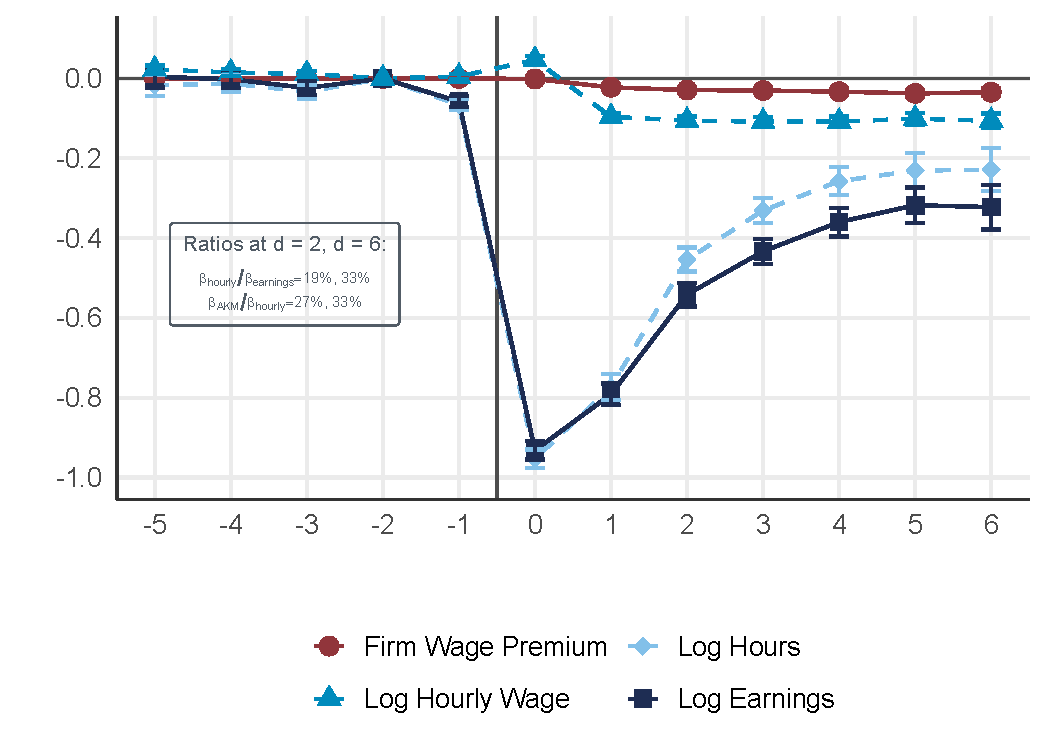
\includegraphics[width=\linewidth, trim={0cm 0cm 0.1cm 0cm}, clip,max width=\linewidth]{figures/01_event_figures/figure_1_le_wage_decomposition.pdf} \\
		\floatfoot{\footnotesize{\textsc{Notes}: This figure reports event-study estimates of the effect of job displacement on log hourly wage, log hours, log earnings and firm-specific wage premium for a sample of workers dismissed for economic reasons (LE)---see equation (\ref{eq:main_estimating_equation}) and associated text for more details on the specification. All estimates are computed on worker-years with positive hours and earnings, i.e.\ conditional on re-employment (see Section \ref{sec:decomposition_losses}). In the text, the ratios $\beta^{\text{AKM}}/\beta^{\text{earnings}}$ and $\beta^{\text{hourly}}/\beta^{\text{earnings}}$ are equal to the effect on firm-specific premium and hourly wage respectively divided by the effect on overall earnings and represents the fraction (expressed in percents) of total earnings losses due to each effect at $d=2,6$. \textbf{Sample}: The sample contains 8{,}341 individuals laid-off for economic reasons who end-up being re-employed post-displacement. \textbf{Outcomes}: Table \ref{apptab:definitions} provides more details on variables' definition.  Wage premia are estimated, following the AKM framework, as firm-fixed effects in a two-way regression of log-hourly wage on firm and worker fixed effects---see section \ref{sec:data:firm:premium} for more details. \textbf{Additional information}: Table \ref{tab:evstudytable_body} reports coefficients' value. Appendix Table \ref{apptab:evstudy_worker_outcomes} provides more details. \textbf{Standard errors}: robust standard errors clustered at the worker-level; displayed confidence intervals at the 99\% level.	}}
\end{center} \end{figure}


\begin{figure}[h!] \centering
	\caption{Productivity and labor share of current employers\label{fig:ln_apl_ls}}


	\begin{subfigure}[b]{.49\textwidth}
		\centering
		\caption[]{\small Productivity} \label{fig:prod_res_within_btw}
		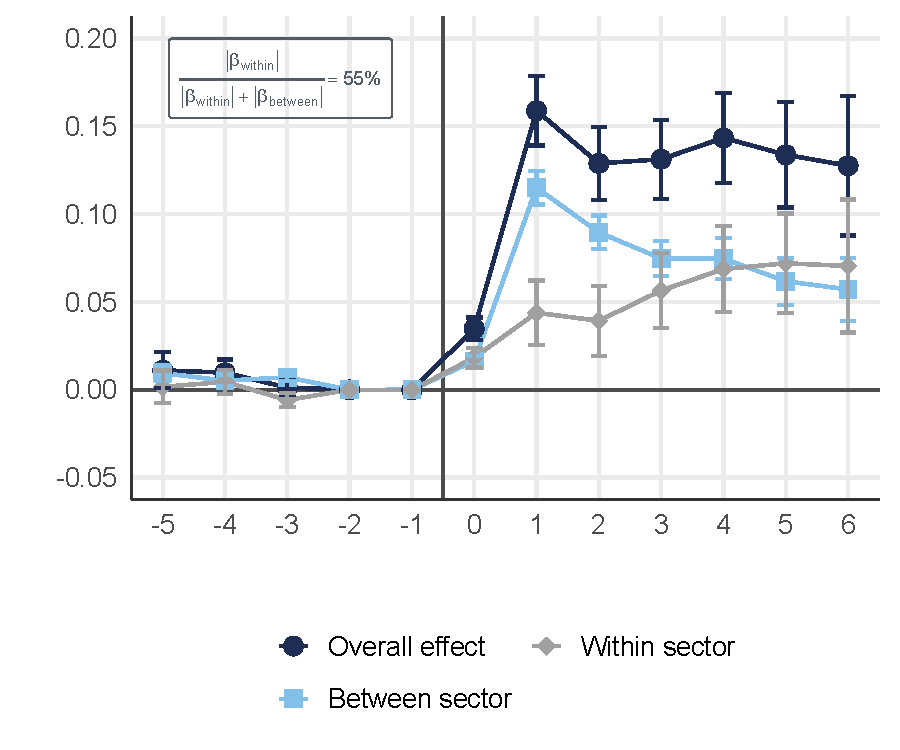
\includegraphics[scale=0.49,max width=\linewidth]{figures/01_event_figures/figure_2_a_productivity.pdf}
	\end{subfigure}
	\begin{subfigure}[b]{.49\textwidth}
		\centering
		\caption[]{\small Labor share of value-added} \label{fig:ln_Lshare_within_btw}
		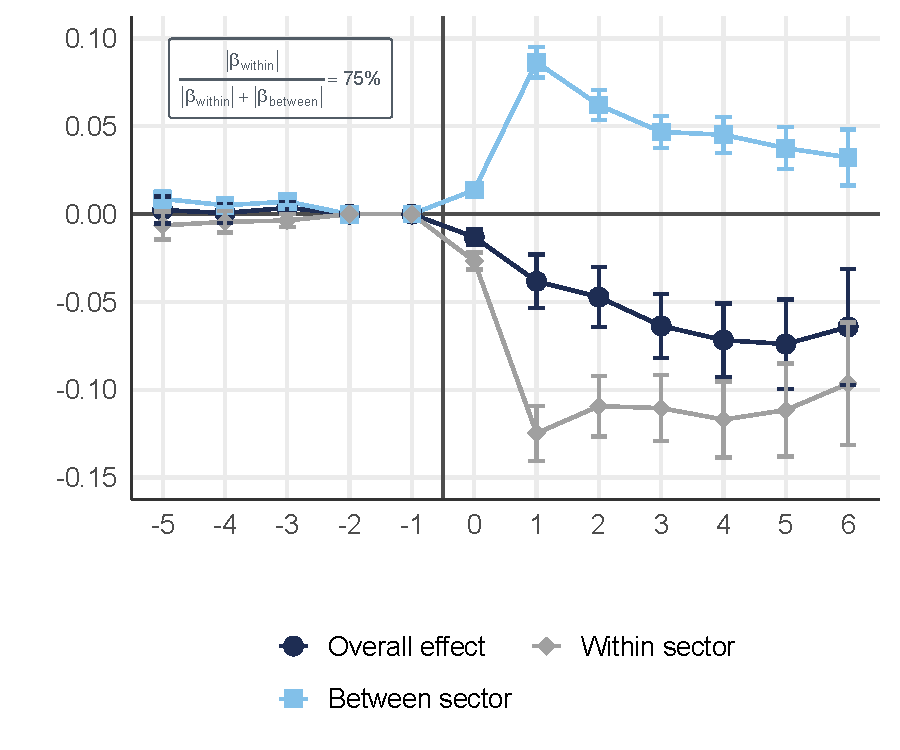
\includegraphics[scale=0.49,max width=\linewidth]{figures/01_event_figures/figure_2_b_labor_share.pdf}
	\end{subfigure}

	\begin{subfigure}[b]{.49\textwidth}
	\caption{Firm Wage Premium} \label{fig:firm_fe_within_btw}
	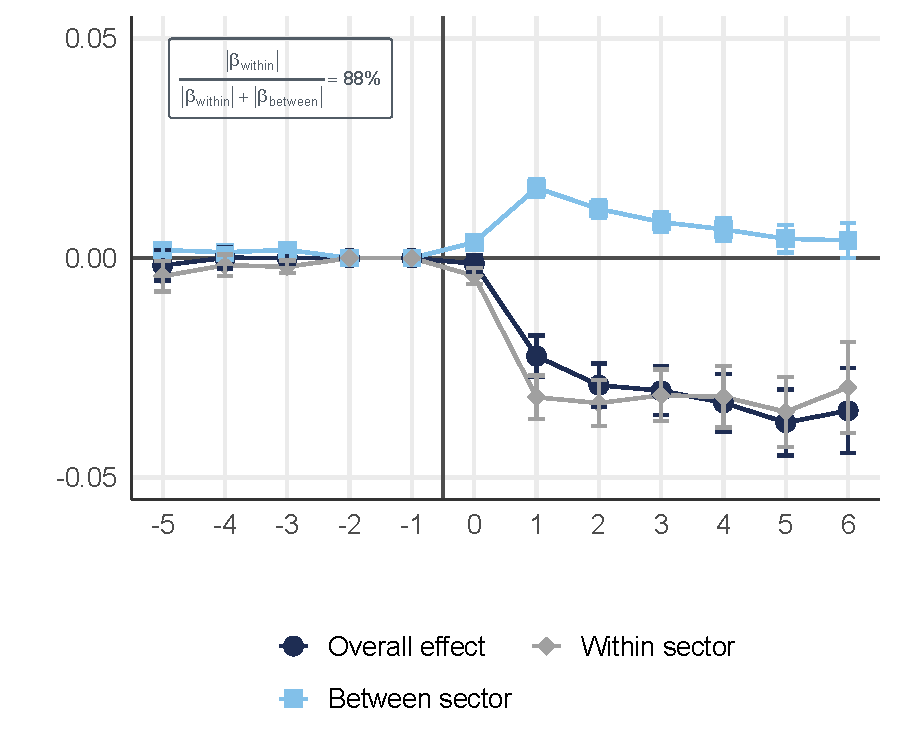
\includegraphics[width=\linewidth,max width=\linewidth]{figures/01_event_figures/figure_2_c_firm_premium.pdf}
	%	\floatfoot{\footnotesize{\textsc{Notes}: The sample contains 9,251 economic dismissals. 99\% confidence interval are displayed, based on robust standard errors clustered at the worker-level. The specification includes individual and year fixed-effects, see equation (\ref{eq:main_estimating_equation}) and associated text for more details. 
	%			Productivity is computed as the residual of a regression of value-added onto tangible capital and employment during the period 2001-2004.}}
\end{subfigure}


	\floatfoot{\footnotesize{\textsc{Notes}: 
			This figure reports event-study estimates of the effect of job displacement on the reallocation of workers towards firms with varying levels of productivity, value added per workers and labor share. Coefficients are obtained by estimating the specification of equation \ref{eq:main_estimating_equation} where the dependent variable is sequentially productivity, value added per worker and labor share. \textbf{Sample}: The sample contains 8,341 individuals laid-off for economic reasons who end-up being re-employed post-displacement. Productivty can be estimated for only 7,524 of those. \textbf{Comment on timing}: Firm-level outcomes are computed as three-year averages centered on $t^D-4$ (i.e.\ over $t^D-5$, $t^D-4$, and $t^D-3$), while displacements occur from 2005 to 2012. Accordingly, event-study coefficients reflect the movement of workers to firms with different initial characteristics and \textit{not} within-firm changes. \textbf{Definition of firm-level outcomes}: See Table \ref{apptab:definitions} for details. Productivity is the residual of an OLS regression of value-added on tangible capital and labor with year fixed effects. The labor share is computed as total labor cost over value-added. In lighter shade, we display the coefficients using a decomposition each of these variables as well as the AKM fixed-effect into a sectoral average at the 3-digit level (between sector $\bar{y}_s$ ) and a deviation from the sectoral average (within sector $R_i=y_i - \bar{y}_s$). The relative size of the within effect is computed as the absolute value of the within effect divided by the sum of the absolute value of the two effects, $|\beta_{\text{within}}| / (|\beta_{\text{within}}|+|\beta_{\text{between}}|)$, evaluated at the latest available horizon for each outcome: $t^D+5$ for productivity (where firm-level balance-sheet data are available only through that horizon) and $t^D+6$ for the labor share and the AKM firm wage premium. \textbf{Additional information}: Table \ref{tab:evstudytable_body} reports coefficients' value. Appendix Table \ref{apptab:evstudy_firm_outcomes} provides more details. \textbf{Standard errors}: robust standard errors clustered at the worker-level; displayed confidence intervals at the 99\% level.}}
\end{figure}

%, where value-added is deflated using 2-digit value added deflator (\textit{Indice de prix de la valeur ajoutée brute par branche})

%The sample contains 10,336 economic dismissals. 99\% confidence interval are displayed, based on robust standard errors clustered at the worker-level. The specification includes individual and year fixed-effects, see equation (\ref{eq:main_estimating_equation}) and associated text for more details. 

\begin{figure}[h!] \centering
	\caption{Quality of labor relations: firm-level measures  \label{fig:LE_accords}}
	%\caption{Firm-level collective agreements \label{fig:LE_accords}}
	\begin{subfigure}[b]{.49\textwidth}
		\centering
		\caption[]{\small Indicator of wage agreement (2005-2007)} \label{fig:LE_acc_main}
		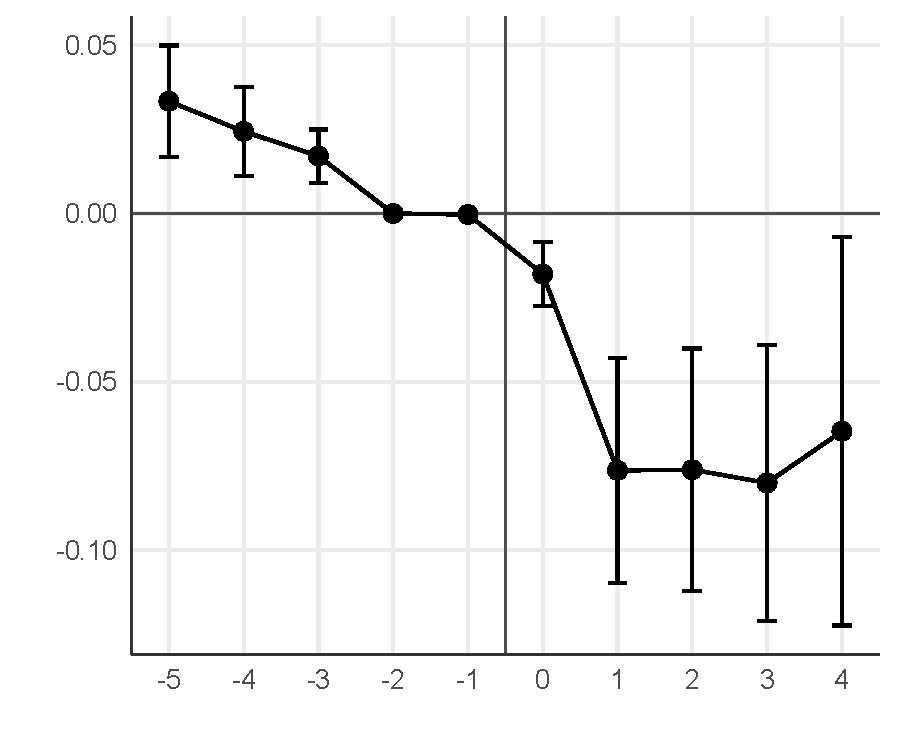
\includegraphics[width=\linewidth,max width=\linewidth]{figures/01_event_figures/figure_3_a_wage_agreement.pdf}
	\end{subfigure}
	\begin{subfigure}[b]{.49\textwidth}
		\centering
		\caption[]{\small Election turnout} \label{fig:LE_elec_main}
		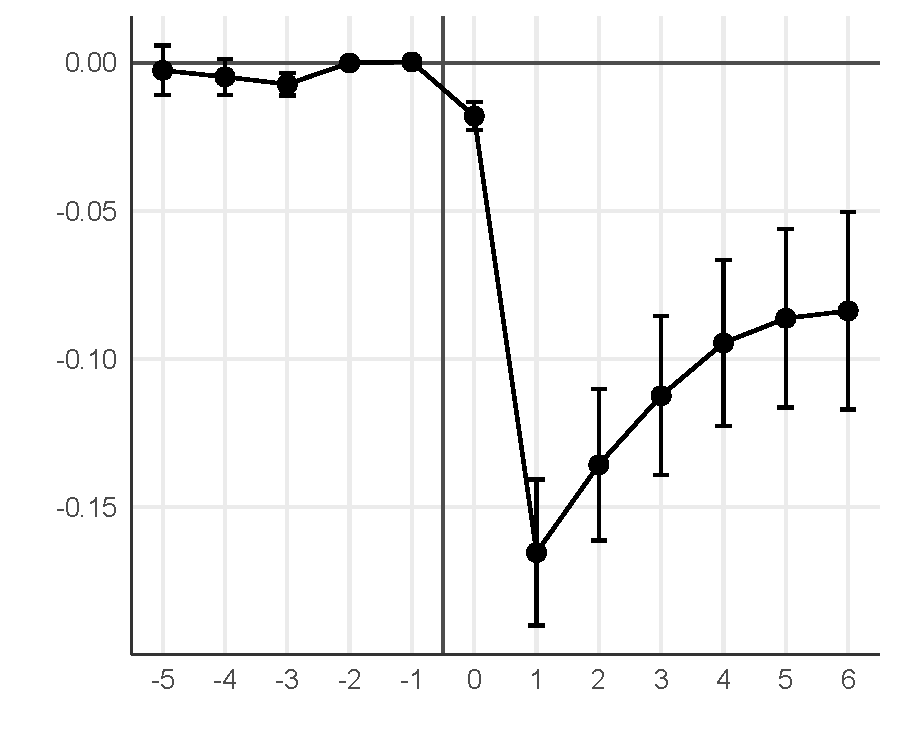
\includegraphics[width=\linewidth,max width=\linewidth]{figures/01_event_figures/figure_3_b_election_turnout.pdf}
	\end{subfigure}
	
	\floatfoot{\footnotesize{\textsc{Notes}: This figure reports event-study estimates of the effect of job displacement the reallocation of workers towards with varying propensities to conclude collective agreements (panel \ref{fig:LE_acc_main}) and turnouts at professional elections (panel \ref{fig:LE_elec_main})---see equation (\ref{eq:main_estimating_equation}) and associated text for more details on the specification. \textbf{Definition of the outcomes:} The dependent variable pertaining to collective agreements is an indicator equal to 1 when firms signed at least one agreement related to wages over the period 2005 to 2007. Because we restrict the focus to LE laid-off post 2007, we do not observe individuals after $t^D+4$. The variable on firm's average turnout at workplace election is computed based on elections taking place over 2009-2012. More details are provided in Section \ref{sec:Nego}, and Table \ref{apptab:definitions} provides more details on variables' definition. \textbf{Comment on timing:} Each firm is associated with a single value of each outcome, so that event-study coefficients reflect reallocation of workers between firms and not within-firm changes in such outcomes.
	\textbf{Additional information}: Appendix Tables \ref{tab:nego:LEnego_acc_result} and \ref{tab:nego:LEnego_ele_result} provide detailed results.
	\textbf{Standard errors}: robust standard errors clustered at the worker level; displayed confidence intervals at the 99\% level.}} 
\end{figure}

